\chapter{Part I: Rainbow Options}
Developer: Yann Renoux

\noindent Validator: Simon Leger


%DEVELOPER WRITES THIS PART --->

\section{Requirements}

In this section, we wrote an object that represents the characteristics and behavior of rainbow options with an eye towards extending to more than 2 assets and a variety of pay off functions. as such, our object was supposed to report for 2 assets:
\begin{itemize}
	\item S1 and S2 are prices of asset 1 and asset 2 at exercise
	\item W1 and W2 are the respective weights
	\item K is the strike
	\item M is a multiplier 1=CALL, -1=put
	\item Spread Option max \{M * (W1*S1 � W2*S2-K), 0\} - Type SpreadOptionMax in the class
	\item 2-asset basket max \{M * (W1*S1 + W2*S2-K), 0\} - Type AssetsBasketMax in the class
	\item Best Of 2 assets and cash max \{W1*S1, W2*S2, K\} - Type BestOf2AssetsCash in the class
	\item Worst Of 2 assets and cash min \{W1*S1, W2*S2, K\} - Type WorstOf2AssetsCash in the class
	\item Maximum Of 2 Assets max \{M * (max[W1*S1 , W2*S2]-K), 0\} - Type Max2AssetsCall / Max2AssetsPut in the class
	\item Minimum Of 2 Assets max \{M * (min[W1*S1 , W2*S2]-K), 0\} - Type Min2AssetsCall / Min2AssetsPut in the class
	\item We also added the BetterOf2Assets / WorseOf2Assets, which is basically the BestOf2AssetsCash / WorstOf2AssetsCash with a strike equal to 0.
\end{itemize}

As we really had an eye towards more than 2 assets, we do not take a single correlation as parameter, rather a correlation matrix on which we perform Cholesky decomposition to correlate the normal samples (see next section). Of course a default constructor with a "Real" as correlation has been implemented. The object uses any set of weights -- they need not be equal to 1 in sum, as the option can provide leverage or low exposition, a volatility surface for each stock and a single yield curve. Indeed we have made the choice not to consider for now quanto options, so each stock having the same currency, there need not be more than one yield curve.

This framework activelly uses the Monte Carlo Engine, but we discovered some interesting things as for which random number generator to use, and how to use it efficiently.




You will write an object allows you to simulate stock prices in the future. This object should take a list of underlying stock assets, volatility surfaces and correlation matrices and be able to get simulated prices for each stock at any time T.
Using the two assets provided, implement the rainbow options described above.
Write methods to
Compute the fair market value of the option.
Compute partial delta, partial gamma and partial vega with respect to the two assets.
Compute a measure for Correlation Risk for any pair of assets i.e. a change in price of the option for a change in correlation between the 2 assets.
Validate your model using closed form solutions wherever applicable.
As part of your report, describe your test cases, results and a graph the difference between prices and greeks obtained using closed form and prices obtained using simulation.

\section{Design }


We have already explained the payoff types we implemented, and to check our prices we used the closed forms when it was applicable. Rubinstein wrote in 1991 and 1995 in "Somewhere Over the Rainbow" and "Return to Oz" that spread options, basket options and dual-strike options do not have a closed form. Also, for the Worst Of 2 Asset plus Cash we were not able to derive a closed form, but there should be one. As for the other types of rainbow options, we refered to the web-site \textit{http://www.global-derivatives.com/options/rainbow-options.php} to get them. For these the weights are taken equal to 1 for each stock, and for the Best Of Cash/Worst Of Cash/Better/Worse, the multiplier is equal to 1. The closed forms use the following variables with usual notations:
\begin{eqnarray*}
	\s_A&=&\sqrt{\s_1^2+\s_2^2-2\r\s_1\s_2}\\
	\r_1&=&\frac{\r\s_2-\s_1}{\s_A}\\
	\r_2&=&\frac{\r\s_1-\s_2}{\s_A}\\
	d_1&=&\frac{\ln\left(\frac{S_1}{K}\right)+(r-q_1+\frac{1}{2}\s_1^2)T}{\s_1\sqrt{T}}\\
	d_2&=&\frac{\ln\left(\frac{S_2}{K}\right)+(r-q_2+\frac{1}{2}\s_1^2)T}{\s_2\sqrt{T}}\\
	d_3&=&\frac{\ln\left(\frac{S_1}{S_2}\right)+(q_2-q_1+\frac{1}{2}\s_A^2)T}{\s_A\sqrt{T}}\\
	d_4&=&\frac{\ln\left(\frac{S_2}{S_1}\right)+(q_1-q_2+\frac{1}{2}\s_A^2)T}{\s_A\sqrt{T}}\\
\end{eqnarray*}

Now if we denote by $\mathcal{N}$ the cumulative normal distribution and $\mathcal{BN}$ the cummulative bivariate normal distribution, both approximated using Hull's coefficients (see Chapter "Common"), we define:
\begin{eqnarray*}
	A&=&S_1e^{-q_1T}[\mathcal{N}(d_3)-\mathcal{BN}(-d_1,d_3,\r_1)]\\
	B&=&S_2e^{-q_2T}[\mathcal{N}(d_4)-\mathcal{BN}(-d_2,d_4,\r_2)]\\
	B&=&Ke^{-rT}\mathcal{BN}(-d_1+\s_1\sqrt{T},-d_2+\s_2\sqrt{T},\r)\\
\end{eqnarray*}

With these inputs we can then get the prices with closed forms:
\begin{center}
\begin{tabular}{c|ll}
	& Type of Rainbow 					  & Closed Form price\\
	\hline
	(1)& Best of 2 Assets Plus Cash & $A+B+C$\\
	(2)& Maximum of 2 Assets Call   & $(1)-Ke^{-rT}$\\
	(3)& Better of 2 Assets 	      & $A+B+C$ (Where $K = 0$)\\
	(4)& Maximum of 2 Assets Put    & $(2)-(3)+Ke^{-rT}$\\
	(5)& Minimum of 2 Assets Call   & EuroBSCall$(S_1)$+EuroBSCall$(S_2)-(2)$\\
	(6)& Worse of 2 assets		      & EuroBSCall$(S_1)$+EuroBSCall$(S_2)-(3)$\\
	(7)& Minimum of 2 Assets Put    & EuroBSPut$(S_1)$+EuroBSPut$(S_2)-(4)$\\
\end{tabular}
\end{center}

From there we understand that we can also check our formulas by synthetizing on with some others and compare. For example, we have priced all of these for several strikes, spots, volatilities and correlations (see test on rainbow) and substracting (2) from (1) gives at $Ke^{-rT}$ at the 5th decimal for closed form and the second for Monte Carlo. The other combinationes were tested too and are in agreement. See the Monte Carlo later in this chapter to see how we made sure our tests were consistent.

To generate two correlated brownian motions $(X_1,X_2)$, we have to sample 2 normal distributions $(N_1,N_2)$ and do the following:
\begin{eqnarray}
	X_1&=&N_1\\
	X_2&=&\r N_1+\sqrt{1-\r^2}N_2
\end{eqnarray}

In higher dimension, we use the Cholesky decomposition for a correlation matrix $\S$ for $n$ brownian motions, we write $$\S=U^TU$$ where $U$ is a lower triangular matrix. Then 
$$\left(
\begin{array}{c}
X_1 \\
\\
\vdots\\
\\
X_n \\
\end{array}
\right)= U \left(
\begin{array}{c}
N_1 \\
\\
\vdots\\
\\
N_n \\
\end{array}
\right)
$$

The 2 dimension formula is a special case of the Cholesky decomposition with 
$$\left(
\begin{array}{cc}
1 &\r\\
\r&1
\end{array}
\right)
$$

\section{Approach}

As mentionned earlier, a rainbow option has one of the 10 types we defined, but others can be added. We chose not to have an abstract class Rainbow and have 10 other ones inheriting as it would entail repetitive methods for the prices as all the closed forms use the same inputs/outputs. Then we would have put them in the abstract class, but then the inheriting one would have a getPrice() method to assemble the pieces and that would be all. 

It takes a valarray of spot prices, of volatility surfaces, of weights, a multiplier, a correlation matrix and a yield curve, as well as start and end date. Default constructors for lighter creation have been used, such as just specifying two volatilities to maturity, two spots, a single correlation -- and by default weights are equal to 0.5 and the multiplier to 1.

The type can be accessed and changed so as not to have to re-create a whole object. As we have 2 pricing methods, the user can choose whether to use the closed form or Monte Carlo. By default it is the closed form and if there is not, the program automatically switches to Monte Carlo. It goes the same for the greeks. We used a default number of simulations of $100,000$ and got rather good results. Of course the user can specify the number of paths.

The only public methods are the setType, getPrice, and all the greeks, the rest is private. The Rainbow Object call by itself the needed parameters, either the closed form variables mentionned above (computed once and for all and stored, unless we change some characterisitcs), or the Monte Carlo engine. 

\section{Unit tests}

We had to be very, very careful in using random number generators. Indeed we never used the C++ based one and usually used Sobol in one dimension. The main issue with Sobol in one dimension is that the samples are correlated, as it works by dichotomy in the interval. Hence at first we noted the set of differences in prices form Monte Carlo to closed form (Best Of) (fig 8.1)

\begin{figure}
\begin{center}
        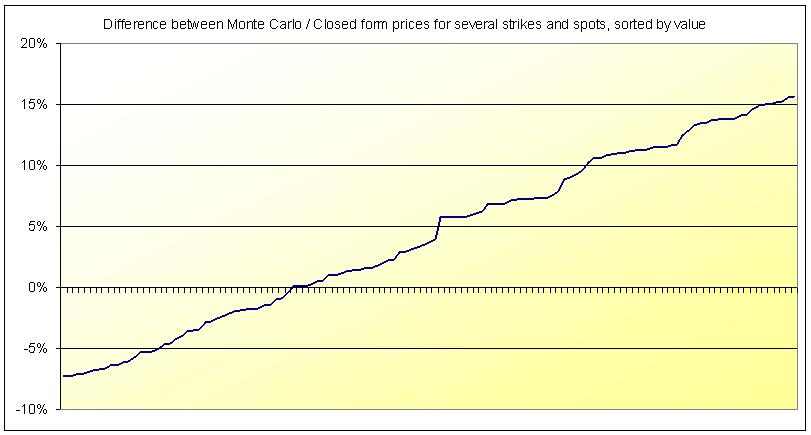
\includegraphics[width=14cm]{sobol.jpg}
        \caption{Prices differences using Sobol for best of's - Strikes and Spot moving between 50 and 150}
\end{center}
\end{figure}

This is of course unacceptable. We can refer to the article of Lee and Huang (Aletheia University) "Pricing Rainbow Options Using Monte Carlo Simulation - 2005" where they tested several random generators to price rainbows with Monte Carlo and showed that Sobol is not the best one to use, even in dimension 2 as it creates aggregates in some spaces of the unit cirle of $\mathbb{R}^2$.

We used VBA to price by Monte Carlo the rainbow and realized we had the correct prices with respect to the closed form. Moving to Mersenne Twister, we have (fig 8.2)

\begin{figure}
\begin{center}
        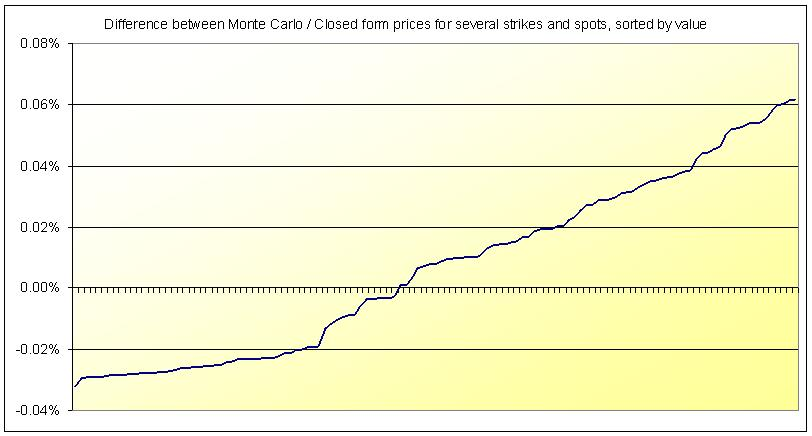
\includegraphics[width=14cm]{mersenne.jpg}
        \caption{Prices differences using Mersenne Twister for best of's - Strikes and Spot moving between 50 and 150}
\end{center}
\end{figure}

The differences do not exceed 8 basis points in relative absolute value, which is a very good thing.

We now had another issue. Indeed as we did not do the calculus for exact closed form value concerning the greeks, the method is finite difference. But Monte Carlo by itself converges to the prices but two different runs can lead to different prices. Hence assume the following: one it 2bps lower than the closed form and the other is 4 bps higher. Hence the greek calculation would be totally off. To calculate the greeks while bumping the reference parameter (spot, volatility, rate, etc) up and down, we have to make sure each set of paths faces the same states of the world, i.e. the same random samples, else it is completely off. We noted some deltas that should be 17 with closed form and that were swinging beween 5 and 500 depending on when we calculated them. We have to reset the seed of the random generator each time we use the engine, so as to make sure if we price exactly the same product with Monte Carlo, we get to exactly the same price. This has been done and here are the distribution of differences for the partial delta for the Best of, the Max Call and the Min Put (fig 8.3, 8.4 and 8.5).

\begin{figure}
\begin{center}
        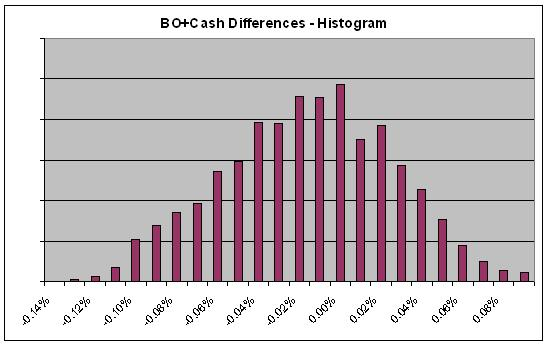
\includegraphics[width=14cm]{BOCPriceDiff.jpg}
        \caption{Distribution of delta differences Monte Carlo/Closed Form for the Best of, for different spots and strikes}
\end{center}
\end{figure} 

\begin{figure}
\begin{center}      
        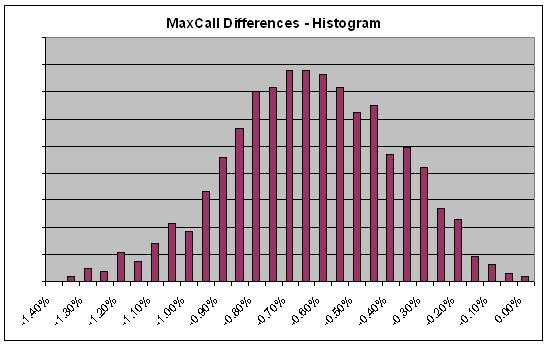
\includegraphics[width=14cm]{MaxCallPriceDiff.jpg}
        \caption{Distribution of delta differences Monte Carlo/Closed Form for the Max Call, for different spots and strikes}
\end{center}
\end{figure} 
  
\begin{figure}
\begin{center}    
        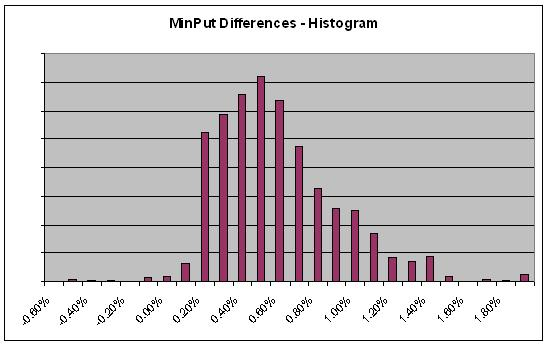
\includegraphics[width=14cm]{MinPutPriceDiff.jpg}
        \caption{Distribution of delta differences Monte Carlo/Closed Form for the Min Put, for different spots and strikes}
\end{center}
\end{figure}

At the end we have a very reliable object which the user can trust. As an example, here are a set of results we have for some products, and some prices as functions of the strike.

\begin{figure}
\begin{center}    
        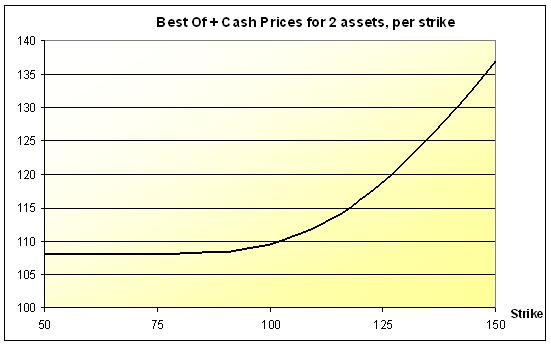
\includegraphics[width=14cm]{BOCPRice.jpg}
        \caption{Best of price as a function of the strike: $T=1$, $\s_1=\s_2=20\%$, $r=10\%$ and $S_1=S_2=100$}
\end{center}
\end{figure}

The very interesting noticeable fact is the importance of the rho as the strike gets higher. Indeed, in expectation, the stock prices in this case are $S_ie^{rT}\approx 110.5$, hence as we get tho higher strikes, the structure is likely to be close to a zero coupon bond, and be worth the discounted value of the strike. But then, the only risk we have on the product is a rate risk as we are virtually holding a ZCB. And holding a ZCB is being short the rates, meaning if rates move up, our structure is away from the fair value on the downside, and we are loosing money (fig 8.7).

\begin{figure}
\begin{center}    
        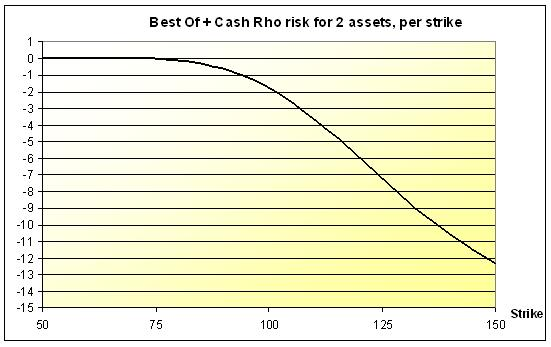
\includegraphics[width=14cm]{BOCRho.jpg}
        \caption{Best of rho as a function of the strike: $T=1$, $\s_1=\s_2=20\%$, $r=10\%$ and $S_1=S_2=100$}
\end{center}
\end{figure}

We also graphed the prices per strike in the same set of inputs for the 2 assets MAx/Min Call/Put's (fig 8.8)

\begin{figure}
\begin{center}    
        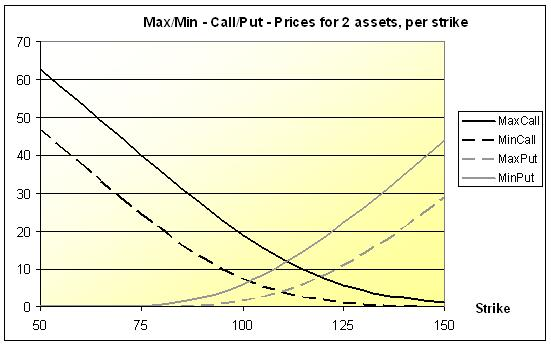
\includegraphics[width=14cm]{MAXMINCALLPUT2.jpg}
        \caption{Max/Min Call/Put's as functions of the strike: $T=1$, $\s_1=\s_2=20\%$, $r=10\%$ and $S_1=S_2=100$}
\end{center}
\end{figure}

As a set of results for the Best Of plus Cash, the MaxCall and the MinPut, we have run the Closed Form pricing range for the greeks, for a 2Y rainbow with $5\%$ interest rate. As both weights are identical, the partial with respect to both assets are equal. For the range of parameters, spots and strikes move in $[80,120]$, correlation in $[-1,1]$ and volatilities in $[10\%,30\%]$ The results are shown in table 8.9.

\begin{figure}
\begin{center}  
\begin{tabular}{|l|l|l|l|l|l|l|}
\cline{3-7}
\multicolumn{1}{l}{} &  & \multicolumn{1}{c|}{Partial Delta} & \multicolumn{1}{c|}{Partial Gamma} & \multicolumn{1}{c|}{Partial Vega} & \multicolumn{1}{c|}{Rho} & \multicolumn{1}{c|}{Correl} \\ 
\hline
Best Of & Min & \multicolumn{1}{r|}{0.32} & \multicolumn{1}{r|}{0.00} & \multicolumn{1}{r|}{0.01} & \multicolumn{1}{r|}{-42.39} & \multicolumn{1}{r|}{-16.40} \\ 
\cline{2-7}
 & Max & \multicolumn{1}{r|}{109.53} & \multicolumn{1}{r|}{520.09} & \multicolumn{1}{r|}{18.74} & \multicolumn{1}{r|}{0.00} & \multicolumn{1}{r|}{10.45} \\ 
\hline
MaxCall & Min & \multicolumn{1}{r|}{0.00} & \multicolumn{1}{r|}{0.00} & \multicolumn{1}{r|}{0.06} & \multicolumn{1}{r|}{8.84} & \multicolumn{1}{r|}{-15.59} \\ 
\cline{2-7}
 & Max & \multicolumn{1}{r|}{116.93} & \multicolumn{1}{r|}{519.42} & \multicolumn{1}{r|}{18.91} & \multicolumn{1}{r|}{28.28} & \multicolumn{1}{r|}{7.84} \\ 
\hline
MinPut & Min & \multicolumn{1}{r|}{-61.63} & \multicolumn{1}{r|}{0.10} & \multicolumn{1}{r|}{0.02} & \multicolumn{1}{r|}{-21.71} & \multicolumn{1}{r|}{-16.40} \\ 
\cline{2-7}
 & Max & \multicolumn{1}{r|}{0.00} & \multicolumn{1}{r|}{192.37} & \multicolumn{1}{r|}{4.33} & \multicolumn{1}{r|}{-2.29} & \multicolumn{1}{r|}{3.82} \\ 
\hline
\end{tabular}
	\caption{A few results on the greeks - Min and Max values noticed for reasonable parameters}
\end{center}
\end{figure}

It confirms the general intuition in which of course the Best of works as a call so it is long delta like the call, the put being short delta. All these are long gamma, as the single stock european versions, as well as long vega, which is understandable as when you own them, if the implied volatility goes up, their value appreciates. The rho is also logical: short for the best of + cash as explained, long for the call and short for the put, as for the european Black-Scholes options. And as for the correlation, depending on whether one spot is higher than the other, and whether their base correlation is positive or negative, the correlation risk can have a positive or a negative impact. Indeed, say we have a Max Call, if the base correlation is positive and high, the maximum is likely to be higher, so is the price: when the correlation decreases, it decreases the price.

Track of the results can be found in the data directory in rainbow2\_yann.xls, rainbow\_MC\_yann.xls and resRainbow\_yann.xls.

\section{Choices}
%<any important design choices you made, e.g. data structures, class hierarchy, algorithm, etc. and a justification for the decision>

We chose not to use dividends in the whole project (from Black-Scholes to the rainbows), but we could easily add them in our closed forms as shown earlier, and to Monte Carlo by adjusting the drift class and removing the dividend rate from the risk free growing rate. We had to amend the Drift/Gaussian/Random/MCEngine/Payoff classes in default constructors so as to avoid passing valarrays all the time and be more efficient: with non path dependant options, the only simulated point is the terminal one, so a one period model does not need to pass arrays of one parameter.

The choice was made to enable $n$ assets, so that adding a new type does not change the whole stucture of the class, and just needs adding the relevant pricing method to the class.




\section{Validation}


\subsection{Approach}

%<i.e. what alternate method was used to validate the results - if this required a lot of code then similar outline as above should apply>
To validate the results of this part even further, the only possibility was to recreate a monte carlo pricer with an easire structure, 
making it easier not to make bugs inside. For this we chose to dewvelop it in VBA. Since we also had closed formulas for some options 
we were quite confident with the results of our C++ pricer, but for some options, it was comfortable to get the same results with 
another pricer. This pricer can be found in the data part of our project under the name RainbowMCTests\_simon.xls. 
The user can input his own parameters in the spreadsheet, choose the number of simulations to run, a maximum acceptable error and 
can then run the simulation. One has to be careful since the program is much slower in VBA. After the calculation is finished 
there is a cell indicating TRUE on a yellow background if all tests passed or FALSE on a red background if some failed. We were happy 
to check that all results were really good and very close to our c++ results, even for a small number of generations.


%<i.e. what bugs were found>
